%コンパイル方法: opt+cmd+b → opt+cmd+v
\RequirePackage{plautopatch}

\documentclass[a4paper, 9pt]{ltjsarticle}


% マージン設定
\usepackage[top=20mm, bottom=25mm, left=20mm, right=20mm]{geometry}

% LuaLaTeX用日本語対応パッケージ
\usepackage{luatexja}
\usepackage{luatexja-fontspec}

% 必要なパッケージ
\usepackage{fontspec}
\usepackage{titlesec}
\usepackage{graphicx}
\usepackage{amsmath}
\usepackage{amssymb}
\usepackage[hidelinks]{hyperref}
\usepackage[english, japanese]{babel}
\usepackage{multicol} % 二段組用パッケージ
\usepackage{indentfirst}
\usepackage{tikz} % カスタム点線用
\usepackage{authblk} % 著者・所属パッケージ
\usepackage{here}
\usepackage{caption}
\usepackage{bookmark}
\usepackage{array}
\usepackage{booktabs}
\usepackage{diagbox} % 斜線を入れるためのパッケージ
\usepackage{caption}
\usepackage[super]{cite}
\renewcommand\citeform[1]{[#1]}

\captionsetup{labelsep=space}


% \setmainfont[Ligatures=TeX]{Times New Roman}
% \setmainjfont[BoldFont=MS Gothic]{MS Mincho}

\renewcommand{\baselinestretch}{0.95}
\renewcommand{\labelenumi}{(\arabic{enumi})}

% セクション見出しのカスタマイズ
\titleformat{\section}
  {\fontsize{10pt}{10pt}}
  {\thesection.}
  {1em}{}

\titleformat{\subsection}
  {\fontsize{10pt}{10pt}}
  {\thesubsection}
  {1em}{}

\titleformat{\subsubsection}
  {\fontsize{10pt}{10pt}}
  {\thesubsubsection}
  {1em}{}

  \setlength{\parindent}{1em}
% \setlength{\belowcaptionskip}{1em} % キャプション下の余白を -10pt に設定


%section前に余白を作る
\titlespacing*{\section}{0em}{1em}{0em}
\titlespacing*{\subsection}{0em}{1em}{0em}
\titlespacing*{\subsubsection}{0em}{1em}{0em}

\pagestyle{empty}


\begin{document}

\setlength{\columnsep}{7.5mm}

\twocolumn[
    \begin{center}
        {\vspace{-1em}}

        {\fontsize{15pt}{15pt}\selectfont{災害時を想定したアドホックネットワーク構築手法の検討}}

        {\vspace{1.5em}}

        {\fontsize{13pt}{13pt}\selectfont{Study of Construction Methods for Ad-Hoc Network under Disaster}}
    \end{center}



    \begin{flushright}
      {\fontsize{11pt}{11pt}\selectfont{T5-17 末廣隼人\\}}
      {\fontsize{11pt}{11pt}\selectfont{指導教員 髙﨑和之}}
    \end{flushright}

    \vspace{1em}

    \thispagestyle{empty}
]

\section{はじめに} \label{label:first}
日本では地震をはじめ多くの自然災害が発生しており,災害時には通信ネットワークが使えなくなる可能性がある.
そこで,アドホックネットワークを活用し地域限定ながら被災状況の把握や情報伝達を可能とする研究が行われている.
本研究では,人口密度に応じた経路構築方法を考案し,その効果をシミュレーションで検証した.%

\section{理論} \label{label:theory}
\subsection{アドホックネットワーク} \label{sublabel:about ad-hoc network}
アドホックネットワークとは,中央の管理者やルータ,アクセスポイント等の既存のインフラストラクチャを介さずに,端末(以降ノードという)同士が直接通信を行う一時的なネットワークのことである.
遠くのノードと通信を行う場合,隣接する他ノードを中継機として利用し,バケツリレーのようにデータを送信するマルチホップ通信技術を用いる.%
\\ \indent 本研究では,低コスト,低消費電力でスマートフォンに内蔵されているBluetoothモジュールを用いたアドホックネットワークを想定し,
より消費電力が少ないBluetooth Low Energyの接続目安距離である30mを最大通信距離としてシミュレーションを行った.

\subsection{ルーティング制御方法} \label{sublabel:routing control}
各ノードが通信を行う際のルーティング方式には大きく分けてリアクティブ型,プロアクティブ型,ハイブリッド型の3種類がある.
各方式の特徴を次に示す.本研究では,リアクティブ型の考え方を元に経路生成手法の検討を行った.
\begin{enumerate}
  \item \label{reactive} リアクティブ型 \par  
  \indent 通信要求が発生した時に近くのノードとその場でデータのやり取りを行い経路を作成する.
  通信開始までに遅延が生じるが経路情報維持のための通信が不要なため通信頻度の低い環境では消費電力が少なく長時間使用できる.
  代表的なプロトコルとしてAODVやDSRなどがある.

  \item \label{proactive} プロアクティブ型 \par
  \indent 近くのノード間で常に情報をやりとりし経路をあらかじめ作成しておく.あらかじめ経路が作成されているため,通信開始までの遅延が少ない反面,
  定期的にデータのやり取りを行うため消費電力が多い.代表的なプロトコルとしてOLSRやTBRPFなどがある.

  \item ハイブリッド型 \par
  \indent (\ref{reactive}),(\ref{proactive}) の2つを組み合わせたルーティング方式である.代表的なプロトコルとしてはZRPなどがある.
\end{enumerate}

\section{提案手法} \label{label:proposed method}
経路生成のシミュレーションにあたりノードの密度は2024年10月1日現在の日本の人口密度\cite{人口密度}にスマートフォンの所有率88.6\%\cite{スマホ保有率}を乗じた数とした.%
人口密度が高い地域として埼玉県,低い地域として福島県2つの地域に対してシミュレーションを行った.
また,人口密度が低い地域ではノード同士の間隔が大きくなってしまうため,電柱にBLE機能等を有した低コストの機器(以降電柱ノードという)を設置した2つの場合についてのシミュレーションを行った.\par
ノードは1km四方の範囲内に配置し,その中で中心に近いノードをスタートノードとし,そこから一番遠いものをターゲットノードとして経路を探索した.
表1にそれぞれの地域の人口密度とシミュレーションに用いたノードの密度を示す.

\begin{table}[h]
  \centering
  \caption{ シミュレーションの条件}
  \begin{tabular}{c|c|c}
    \specialrule{1.5pt}{0pt}{0pt} % 上端の太線(1.5pt)
       & 埼玉県 & 福島県 \\
      \hline
      人口密度 [人/$\mathrm{km}^2$] & 1930 & 126 \\
      \hline
      ノードの数 [個] & 1710 & 112 \\
      \specialrule{1.5pt}{0pt}{0pt} % 上端の太線(1.5pt)
  \end{tabular}
\end{table}

\subsection{人口密度が高い地域の場合} \label{sublabel:high population density}
% 理由
人口密度が高い地域では全てのノードが1つのアドホックネットワークに接続してしまうと経路の複雑化や冗長化により,通信速度や通信品質の低下が発生してしまう.
これらを解決するために,周辺ノードの密度を用いて接続ノードを制限し経路の単純化を行った.ノードの接続条件を次のように定めた. \par

\begin{itemize}
  \item 上流ノードが下流ノードに対してhelloメッセージと自身のMACアドレスをフラッディングする.
  \item 受信した下流ノードはreplyメッセージと自身のMACアドレスを上流ノードに返す.但し,他ノードと接続済みの下流ノードは上流ノードのhelloメッセージを無視する.
  \item 上流ノードはhelloメッセージの返信数で下流ノードの数を認識する.
  \item 下流ノード数が閾値$X$より大きいなら下流ノードの中からランダムで1つ選択し,そうでないならランダムで2つ,下流ノード数が2以下ならそのノードと接続する.
\end{itemize}

$X$はノード密度の閾値であり,それぞれ2\textasciitilde9の場合についてシミュレーションを行った.\par

ノード密度の閾値が5の場合のシミュレーションの実行結果を図\ref{fig:1}に示す.
図\ref{fig:1}の赤点がスタートノードとターゲットノード,青点は接続可能ノード,
オレンジ点は接続不可能ノード,薄青で塗られている部分は通信可能エリアである.接続されていない青点ノードがいくつかあるが,
これは経路生成時に余ったノードであり,万が一近くのノードが消滅した時の代替として使用される.
\begin{figure}[ht]
  \centering
  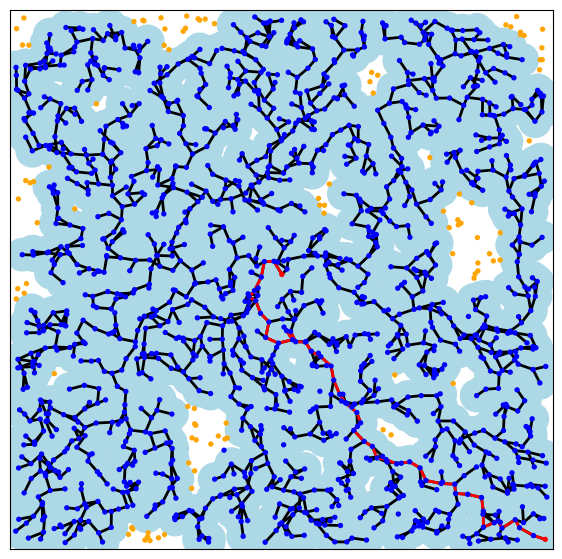
\includegraphics[width=70mm]{シミュレーションの様子.png}
  \caption{人口密度が高い地域のシミュレーション結果(閾値=5)}
  \label{fig:1}
\end{figure}


次に,ノード密度の閾値を2\textasciitilde9に変化させて50回ずつシミュレーションを行い,接続可能ノードをノードの総数で割った接続可能ノード割合の平均値を図\ref{fig:2}
に示した.この図より,閾値が6のとき接続可能ノード割合が73.7\%で一番高くなることが分かった.
\begin{figure}[ht] % [h]は「ここに表示」の意味
  \centering
  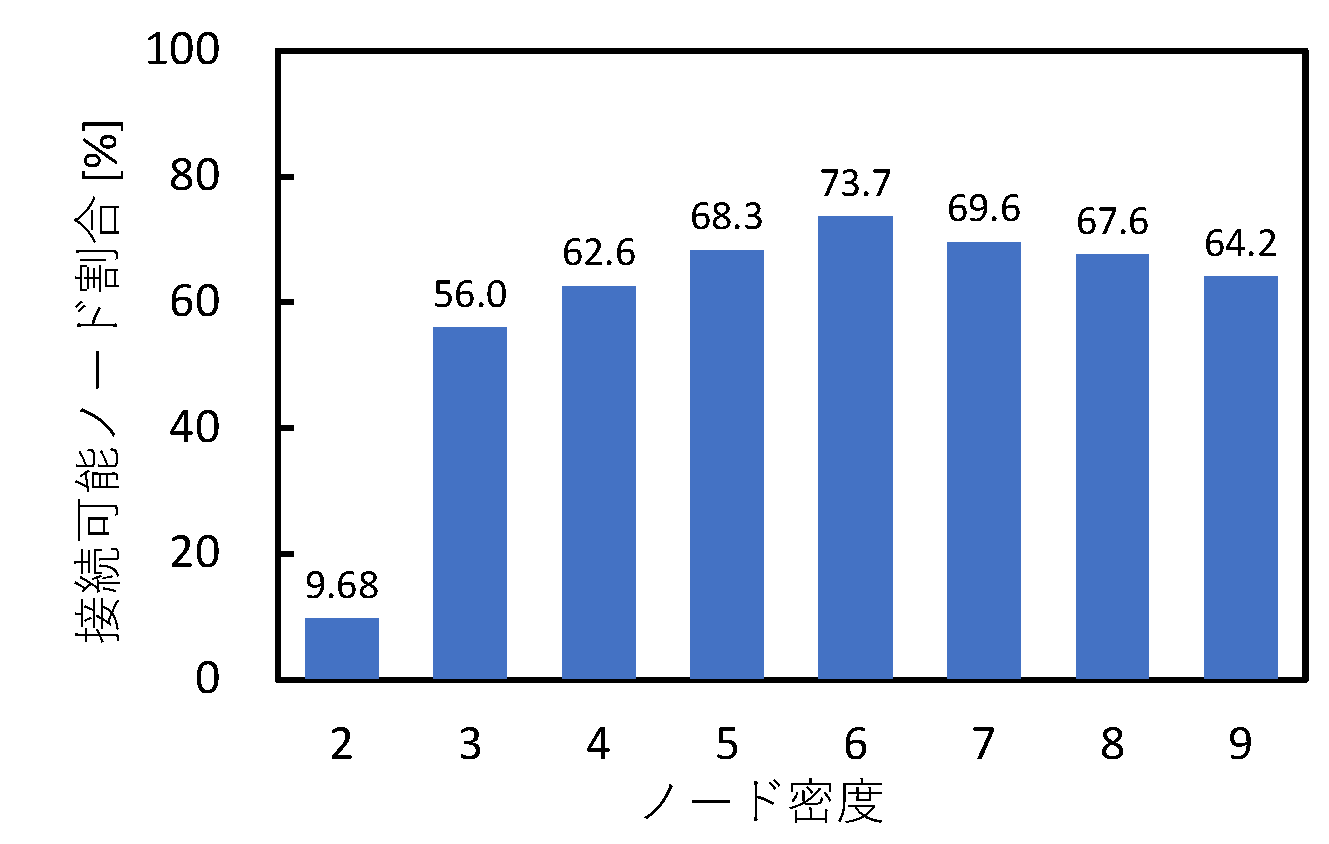
\includegraphics[width=75mm]{提案1の結果.pdf}
  \caption{ ノード密度の閾値に対する接続可能ノードの割合}
  \label{fig:2} % 参照用のラベル
\end{figure}

% \item 人口密度が低い地域の場合 \par
%  紙面の都合上,人口密度が低い地域については結果だけ述べさせていただく.どのノード密度の条件でも接続可能ノード割合は0\textasciitilde5\%の間であった.
% これは,ノードの間隔が大きく偶然近くにいたとしてもその先にノードが存在しないため,ネットワークを広げることができないと考えられる.

\subsection{人口密度が低い地域の場合} \label{sublabel:low population density}
人口密度が高い地域では,ノードのみでアドホックネットワークを構築できたが,人口密度が低い地域ではノード間隔が広すぎるためネットワークのエリアを広げることができなかった.
そこで,電柱ノードを利用することでノードの補完を行った.また,使用するノード密度の閾値は6とした.\par
電柱ノードは次のように定めた.

\begin{itemize}
  \item 電柱ノードは50m間隔で配置\cite{電柱設置間隔}し,電柱ノード間は相互に通信可能であるとした.
  \item 電柱ノードとノードの接続には\ref{sublabel:high population density}節と同様の条件で行う.
\end{itemize}

人口密度が低い地域として福島県の条件を用いた場合のシミュレーション結果を図\ref{fig:3}に示す.
緑点は電柱ノード,その他は図\ref{fig:1}と同じである. \par
ノードの総数を接続が可能なノード数で割った時の接続割合が10回の平均で約99.0\%であった.
\begin{figure}[ht]
  \centering
  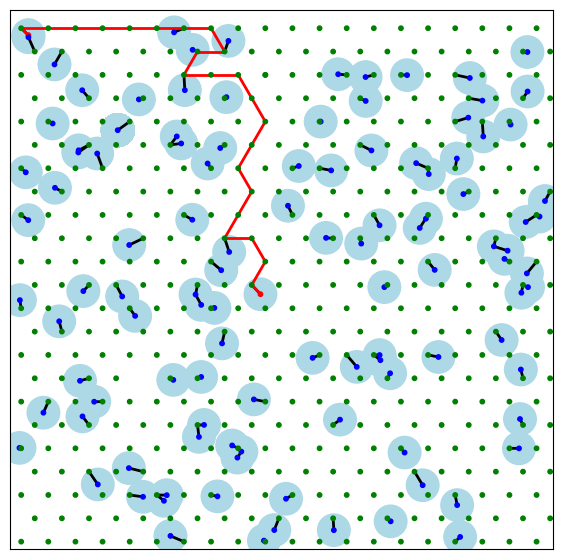
\includegraphics[width=70mm]{電柱を用いたシミュレーション結果.png}
  \caption{ 人口密度が低い地域のシミュレーション結果}
  \label{fig:3}
\end{figure}

\section{考察} \label{label:consideration}
シミュレーションの結果,人口密度が1600人/$\mathrm{km}^2$以上の高い地域ではノード密度の閾値を6にした時が接続可能ノード割合が最も高くなった.
しかし,人口密度が低いエリアが少しでも存在すると電波が届かなくなりネットワークに参加できないという課題が残った.
次に人口密度が低い地域では,ノード間隔が広いためその間を電柱等の公共物にノードを設置して補完を行った.
その結果,ノードの接続可能割合は100\%近くまで上昇した.しかし,電柱の間隔や本数等は実際の環境と比較すると大きく異なったり,
震災状況では電柱が倒壊してしまう可能性があるため,実環境のモデルや電柱の本数を間引いた場合のシミュレーションを行う必要がある.
また,Bluetoothでは通信距離が短く中継端末数が多くなったため,今後は経路探索方法の効率化やIEEE802.11等の中距離通信を用いることで
経路の簡素化を検討する必要があると考えられる.

\section{まとめ} \label{label:conclusion}
本研究では,災害時のアドホックネットワーク構築において,人口密度が高い地域では経路の複雑化やスループットの低下,
低い地域ではノード間距離の問題でネットワーク構築が困難になる課題に対し,
高密度地域ではノード密度の閾値による接続数制限,低密度地域では電柱などの公共物を活用したノード補完を提案し,
簡易な経路生成を実現した.今後は,起伏の多い地形や人口密度の偏りを考慮した実環境シミュレーションを行いたいと考えている.
% 本研究では,災害時を想定したアドホックネットワーク構築する際,多量のノードにより複雑化してしまう経路を
% 下流ノードの接続状況と周辺のノード密度を考慮することにより簡単な経路探索する手法を検討した.
% その結果,周辺ノードの密度が4\textasciitilde6であるとき広範囲なネットワークを生成することができた.
% また,ループが発生しないため通信品質も保つことができると考えられる.しかし,スタートノード周辺のノードの負荷が大きくなってしまうため,
% 複数のスタートノードを用意し,負荷の分散を行う必要があると考えられる.\par
% 今回のシミュレーションでは,アドホックネットワークの技術的課題について触れていないため実際の環境では異なる結果が出ると考えられるため,
% 今後は実環境で実験を行いそれを元にシミュレーションを改良していきたいと考えている.

\begin{thebibliography}{9}
  \bibitem{人口密度} 都道府県市区町村,"都道府県 人口・面積・人口密度ランキング",\url{https://uub.jp/rnk/p\_j.html}.
  \bibitem{スマホ保有率} 総務省,"通信利用動向調査",\url{https://www.soumu.go.jp/johotsusintokei/whitepaper/ja/r04/html/nd238110.html}.
  \bibitem{電柱設置間隔} 東京電力,"全国の「位置情報データ」の代理店販売の概要",\url{https://www.tepco.co.jp/pg/company/press-information/press/2019/pdf/190808j0101.pdf}.
\end{thebibliography}

\end{document}
